\chapter{Background}
\label{chp:chapter_2}

In this chapter, the necessary background information will be covered to be able to fully understand the architecture of the proposed solutions, as well as defining useful terms. 

\section{Wireless Connection}
\label{sec:ch2_wireless_connection}
A wireless connection is a setup between at least two devices. 

Within the Bluetooth Low-Energy specification, there exists a clear hierarchy. In this hierarchy, one device is dominant and is called the Central, and the other side of the connection is with one or more Peripherals. The Central usually takes the shape of a phone or a laptop. These devices include headphones, smartwatches, IoT sensors, push buttons, and more. 

For this thesis, we define three phases for a BLE connection. These phases are:
\begin{itemize}
    \item \textit{Unconnected}: before any connection is established between the Central and the Peripheral
    \item \textit{Connection Setup}: starts from the connection request and ends when the last non-application packet is sent. 
    \item \textit{Application}: starts when connection setup is finished and only application packets are sent. Application packets are packets that are necessary to fulfill the application. 
\end{itemize}
These terms are not officially defined by the BLE specification but are used throughout this thesis. 

\section{Architecture of the Bluetooth Low-energy Stack}
\begin{figure}[]
    \centering
    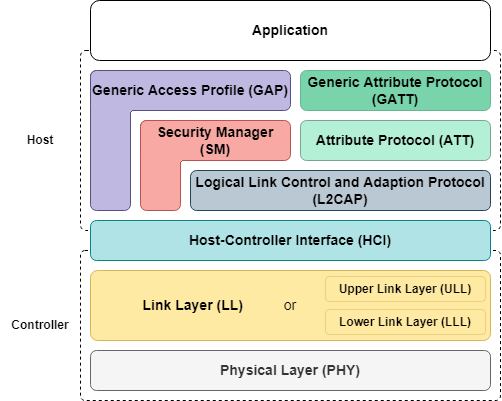
\includegraphics[width=0.8\textwidth,height=6cm,keepaspectratio=true]{images/ble_stack/ble_stack.drawio.png}
    \caption{
        The BLE Network Stack. The controller is comprised of the Physical Layer and the Link Layer. The Generic Access Profile, Security Manager, Generic Attribute Protocol, and Attribute Protocol messages get translated by the Logical Link Control and Adaption Protocol and together form the host. The Host-Controller Interface exists between the host and controller.
    }
    \label{fig:ble_stack}
\end{figure}

As seen in Figure \ref{fig:ble_stack}, the BLE stack is divided into many layers with increasing levels of abstraction. The bottom-most layers, the Physical Layer (PHY) and Link Layer (LL) form the controller, which is responsible for controlling the connection. The top-most layers, the Generic Access Profile (GAP), Security Manager (SM), Generic Attribute Protocol (GAP), and Attribute Protocol (GATT), provide higher level functionality and APIs which, together with the Logical Link Control and Adaption Protocol (L2CAP) form the host.

The separation of the host and controller is derived from how Bluetooth BR/EDR is implemented, where the host and controller can be implemented separately or even exist on different chips entirely. The host and controller are connected together using a Host-Controller Interface. This separation also allows a single radio to be used with a BR/EDR and BLE controller simultaneously and a generic host to support both versions of Bluetooth.

Nordic Semiconductors supplies the SoftDevice for its microcontrollers, which contains the host and controller in a single qualified, pre-compiled binary \cite{nordic_softdevices}. The Zephyr framework can interface with Nordic's SoftDevice Controller through HCI or, since version 3.0.0, supports its own custom Zephyr BLE Controller. Packetcraft implements the entire stack from application to PHY.

\subsection{Physical Layer} The PHY operates at the unlicensed 2.4GHz ISM (industrial, scientific, and medical) band and uses Gaussian frequency-shift keying (GFSK) modulation with adaptive frequency-hopping to reduce collisions. The 2.4GHz band is divided into 40 channels from 2.4000GHz to 2.4835GHz. The radio calculates the next hop using the formula:

\[\text{channel}_{\text{new}} = (\text{channel}_{\text{current}} + \text{hop}) \text{ modulo } 37\]
    
where the value \textit{hop} is exchanged when the connection is established.

BLE has a theoretical maximum throughput of 1Mbps for version 4.2 and 2Mbps for version 5.0. However, in practice, this lies much lower. In normal operation (uncoded), every bit is represented by one symbol. From version 5.0 onwards, BLE supports \textit{Coded PHY} where a single bit is represented by 2 to 8 symbols for improved range but reduced throughput.

\subsection{Link Layer} 
The link layer (LL) directly controls the PHY and manages the link state. The link layer is the only hard real-time layer of the BLE stack and is partly hardware dependent. For this reason, it is usually implemented and kept separate from the rest of the stack. However, Zephyr goes even further and splits the link layer up into an upper and a lower link layer (ULL and LLL respectively), where the ULL is hardware agnostic and generic, and the LLL is hardware specific.

\subsubsection{States and Roles}
\begin{figure}[]
    \centering
    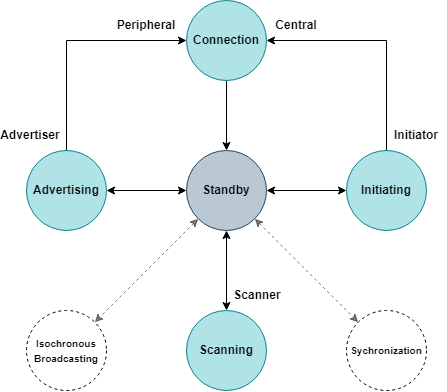
\includegraphics[width=0.8\textwidth,height=6cm,keepaspectratio=true]{images/ll_states/ll_states.drawio.png}
    \caption{
        Link Layer state machine diagram. In the standby state no packets are received or transmitted. Advertisers send advertising packets without a connection, scanners receive advertising packets without the intention of connecting, and initiators initiate a connection with advertisers, which then become the centrals and peripherals, respectively.
    }
    \label{fig:ll_states}
\end{figure}
The link layer can be described as a system of one or more state machines. The states that each LL state machine can occupy are shown in Figure \ref{fig:ll_states}. The link layer should have at least one LL state machine that supports \textit{Advertising} or \textit{Scanning}. 

The link layer in \textit{standby} does not receive or transmit any packets. When the link layer moves from \textit{standby} to \textit{advertising}, the link layer takes on the role of \textit{advertiser}. As an advertiser, the link layer transmits advertising channel PDUs and possibly responds to requests from other devices for more data. The different types of advertising packets and their content will be discussed later.

A link layer in the \textit{scanning} state takes on the role of a \textit{scanner}. In this role, it can listen for advertising packets and consume their content, but it can not form a connection with the \textit{advertiser}.

If a device intends to form a connection with an advertiser, it should enter the \textit{intitiating} state, taking on the role of \textit{initiator}. When an advertisement packet is received, the \textit{initiator} can respond with a \texttt{CONNECT\_IND} packet to form a connection. After a connection is formed, the \textit{initiator} becomes the \textit{central} and the \textit{advertiser} becomes the \textit{peripheral}. The \textit{central} defines the timing of transmission events.

The \textit{synchronization} state is used to listen to periodic advertising trains from a specific device within its \textit{Broadcast Isochronous Group} (BIG). The \textit{isochronous broadcasting} state is used to broadcast data to a group of devices in a BIG. These states are used when a single device continuously streams data to multiple receivers, such as wireless earphones. Figure \ref{fig:ll_states} shows these states with dotted borders since they do not apply to this thesis.

\subsubsection{Advertising and Scanning}
\begin{table}
    \begin{center}
    \begin{tabular}{|l|l|l|l|}
        \hline
        \textbf{Advertising Type} & \textbf{Connectable} & \textbf{Scannable} & \textbf{Directed} \\
        \hline
        \texttt{ADV\_IND} & Yes & Yes & No \\
        \hline
        \texttt{ADV\_DIRECT\_IND} & Yes & No & Yes \\
        \hline
        \texttt{ADV\_NONCONN\_IND} & No & No & No \\
        \hline
        \texttt{ADV\_SCAN\_IND} & No & Yes & No \\
        \hline
    \end{tabular}
    \end{center}
    \caption{Primary advertising packet types.}
    \label{tbl:adv_types}
\end{table}

As an advertiser, the device sends out advertising channel packets at a set interval between 20ms and 10.240ms. The advertiser does this for device discovery, to broadcast data or both. There are four primary types of advertisement packet types. These types are shown in Table \ref{tbl:adv_types}.

These advertisement types can have three traits: \textit{connectable}, \textit{scannable} and \textit{directed}. A connectable advertisement type allows initiators to establish a connection using the \texttt{CONNECT\_IND} PDU. Packet types without the connectable trait are only used to broadcast data.

A scannable advertisement type allows a scanner or an initiator to request more data from the advertiser using a \textit{scan request} or \texttt{SCAN\_REQ} PDU. This forces the advertiser to respond with a \textit{scan response} or \texttt{SCAN\_RSP} PDU, which doubles the amount of data that can be broadcast. In this process the scanner or initiator said to perform \textit{active scanning}. On the contrary \textit{passive scanning} is where the scanner or initiator only listens to advertisement packets and never issues a scan request.

A scanning device can listen for these packets and do nothing, which is called \textit{passive scanning}, or can request more data with a \textit{Scan Request}, which is called \textit{active scanning}. 

Advertising packets can contain up to 31 bytes of advertising data. The structure of the advertising data is shown in Figure \ref{fig:advdata_layout}. The \texttt{AD Type} field is an 8-bit identifier that refers to one of the many predefined advertisement datatypes. This is followed by the length of the data for this type and then the actual data. 

\begin{figure}[]
    \centering
    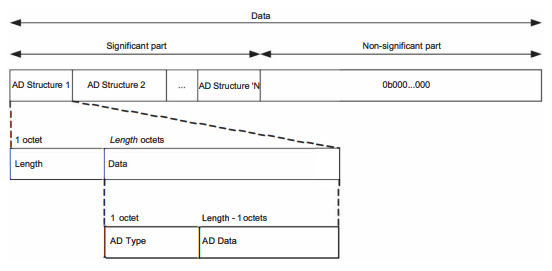
\includegraphics[width=0.8\textwidth,height=6cm,keepaspectratio=true]{images/advertising_data}
    \caption{
        The layout of the AdvData field for advertisement packets. Advertisement packets allow for 31 bytes of consecutive AD Structures. These structures contain the length of the structure, followed by the AD Type, and finally, the AD Data as defined in the specification for that AD Type \cite{bluetooth_spec}.
    }
    \label{fig:advdata_layout}
\end{figure}

\subsubsection{Connection Setup and Parameters}
The connection setup is initiated by the Central by responding with a \texttt{CONNECT\_IND} packet to an advertisement packet. From this moment, a connection between the devices is made, and the setup can begin. The parameters which decide the connection configuration are contained within the \texttt{CONNECT\_IND} packet (\texttt{LLData} field). The most important configuration values to understand are \textit{Connection Interval} (CI) and \textit{Peripheral Latency} (PL). 

\begin{figure}[]
    \centering
    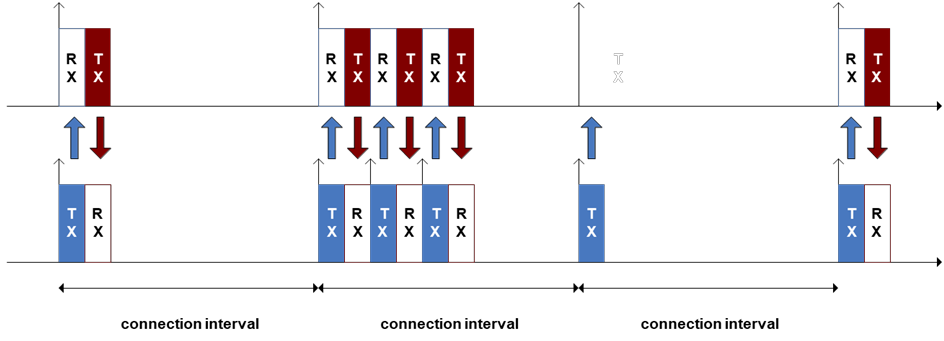
\includegraphics[width=0.8\textwidth,height=6cm,keepaspectratio=true]{images/connection_interval_slave_latency}
    \caption{
        An example timeline of communications between a \color{red} Peripheral \color{black} and \color{blue} Central \color{black}. At every connection interval, a new chain of transmission events can start. This chain can theoretically continue up until the end of the connection interval. If the Peripheral Latency is set to $N$, it allows the Peripheral to skip responding to $N$ connection interval events from the Central to conserve energy. This can be seen in the third spike \cite{nordic_2022}.
    }
    \label{fig:ci_and_pl}
\end{figure}

As you can see in Figure \ref{fig:ci_and_pl}, the Connection Interval is the time between the start of chains of transmit (TX) and receive (RX) events. Multiple TX/RX events can happen within one chain, but when there is no more data to be sent then the current chain is over, and new data can be transmitted at the following interval. Peripheral Latency defines how many Connection Intervals the Peripheral is allowed to skip. For example, take a CI of 2 seconds and a PL of 0. This means that every two seconds, the Central transmits a packet and the Peripheral replies. Now take a CI of 2 and a PL of 1. In this case, the Central transmits every two seconds, but the Peripheral is allowed to sleep every other packet, effectively making the time between transmissions four seconds. 


\begin{table}
    \begin{center}
    \begin{tabular}{|l|l|}
        \hline
        \textbf{Parameter} & \textbf{Constraints} \\
        \hline
        Connection Interval & Range: 0x0006 0x0C80 \\
                            & $Time = N * 1.25ms$ \\
                            & Time Range: 7.5ms to 4000ms \\
        \hline
        Peripheral Latency  & Range: 0x0000 to 0x01F3 \\
        \hline
        Supervision Timeout & Range: 0x000A to 0x0C80 \\
                            & $Time = N * 10ms$ \\
                            & Time Range: 100ms to 32s \\
                            & $Timeout \leq (Latency + 1) * Interval$ \\
        \hline
    \end{tabular}
    \end{center}
    \caption{Connection parameters and parameter constraints.}
    \label{tbl:conn_params}
\end{table}

The units and ranges for the three connection parameters are defined in Table \ref{tbl:conn_params}.

\subsubsection{Feature Expansion and Compliance}
Newer revisions of BLE can add new features to the link layer, adding new functionality or improving throughput. A vendor can also choose not to implement functionality not required for their application to reduce complexity. The supported features are stored in a 64-bit bitmask. The bitmask needs to be exchanged at the beginning of the connection to make sure a controller on one side does not use a procedure that the other controller does not support. Some examples of these features include \textit{LE Encryption} (bit 0), \textit{LE Data Packet Length Extension} (bit 5), \textit{LE 2MB PHY} (bit 11), and \textit{LE Coded PHY} (bit 11), which might sound familiar\cite[p. 2827]{bluetooth_spec}.

A feature that has been mentioned in the list above but not yet addressed is \textit{LE Data Packet Length Extension}. By default, the link layer packet data unit (PDU) allows for 27 bytes of data to be transmitted. The LE Data Packet Length Extension feature allows this to be increased up to 251 bytes for vastly improved throughput. However, higher level protocols like ATT are encapsulated within the LL PDU, so the effective application data per packet will be lower than 251 bytes.

\subsection{Host Controller Interface}
The host controller interface provides a standardized way of communicating between the hardware-specific, real-time part of the stack (controller) and the rest, which is more hardware agnostic (host). The HCI can be implemented as a software API if the host and controller exist within the same silicon or using a hardware interface (UART, SPI, $\text{I}^{2}\text{C}$, USB) when the controller is a separate chip. It is common that the host and controller are implemented on the same chip since that reduces power consumption, which is often a large consideration for BLE devices.

The BLE specification defines a set of standardized HCI commands and events that the host and controller exchange with each other, together with a data packet format and control flow rules\cite{townsend_cufi}. Some vendors choose to extend the functionality of HCI by adding custom commands \cite{ti_ble_dev_guide}, which can allow the developer to control low-level settings of the radio.

\subsection{Logical Link Control and Adaption Protocol}
The task of the Logical Link Control and Adaption Protocol (L2CAP) layer is twofold. First, it encapsulates upper-level protocol packets into the standard LL PDUs, functioning as a multiplexer. The converse of this process is called decapsulation. The second function of L2CAP is fragmentation, which happens when an upper-level protocol packet exceeds the supported LL PDU size and has to be split into multiple L2CAP fragments. The L2CAP layer of the receiving side then has to defragment the packets to create the original packet. L2CAP adds a four byte header to each packet it encapsulates, thus reducing the effective packet data size further from 27 to 23 bytes.

\subsection{Security Manager}
The Security Manager (SM) layer contains both a protocol and a group of security related algorithms and procedures. The algorithms are used to generate security keys which can be distributed using the defined procedures. Afterward, the Security Manager Protocol (SMP) can be used by other layers to safely connect and exchange data.

The following procedures are supported by the Security Manager:
\begin{itemize}
    \item \textit{Pairing} is when a set of temporary security keys are generated to encrypt the link.
    \item \textit{Bonding} can be done after \textit{pairing} by exchanging permanent security keys which are stored in non-volatile memory.
    \item \textit{Encryption Re-establishment} is done to re-use previously stored permanent keys for a new encrypted link without having to \textit{pair} and \textit{bond}.
\end{itemize}

The process of pairing requires the using to confirm the connection by entering a pincode from the peripheral on the central.

\subsection{Generic Access Profile}
The Generic Access Profile (GAP) layer defines the generic procedures related to the discovery of BLE devices and link management aspects of connecting to BLE devices. In addition, it also defines procedures required to attain certain security levels, as well as standard format requirements for parameters that are available at the user level. Most importantly, GAP defines certain \textit{roles} which govern the hierarchy of a BLE network, resulting in the asymmetric power requirements that allow the peripheral devices to operate efficiently.

\subsubsection{Roles}
GAP defines two pairs of roles for a total of four GAP roles. These pairs are the \textit{broadcaster} and \textit{observer} pair, and the \textit{peripheral} and \textit{central} pair.

A broadcaster is a device with a link layer set to advertising, that only transmits data through advertisements of the \textit{non-connectable}. A device in the \textit{broadcasting role} should have a transmitter but a receiver is optional. Devices which are suitable for broadcasting include temperature sensors and locating beacons.

An observer is a device which has its link layer state set to scanning and is only interested in reading advertisement packets without persuing a connection. An observer should have a transmitter but a receiver is optional. Phones are often observers when listening for BLE locating beacons to improve localization accuracy. 

A peripheral (GAP role) is any device which accepts connection requests from other devices. This means any device which is an advertiser, sending out advertisements of the connectable type. When a peripheral (GAP role) goes to the connected link layer state, it changes from an advertiser (LL role) to a peripheral (LL role). A device in the \textit{peripheral role} should have a transmitter and a receiver.

A central (GAP role) is any device which initiates a connection with a peripheral. When central (GAP role) goes to the connected link layer state, it changes from an initiator (LL role) to a central (LL role). A device om the \textit{central role} should have a transmitter and a receiver.

Depending on the application requirements, a device may support multiple roles simultaneously. For example, a phone can be connected with wireless headphones, making it a central, and listening for locating beacons, making it an observer.

\subsection{Attribute Protocol and Generic Attribute Profile}
The Attribute Protocol (ATT) layer allows information to be discovered and transferred between BLE devices in a structured manner. ATT is uses a client/server model, where the data is stored in the ATT server as attribute, and the client performs requests to read or manipulate the attribute data. Each attribute contains a known UUID which is used to identify the type of data contained in the attribute, and a 16-bit handle to identify the attribute itself. 

\begin{figure}[]
    \centering
    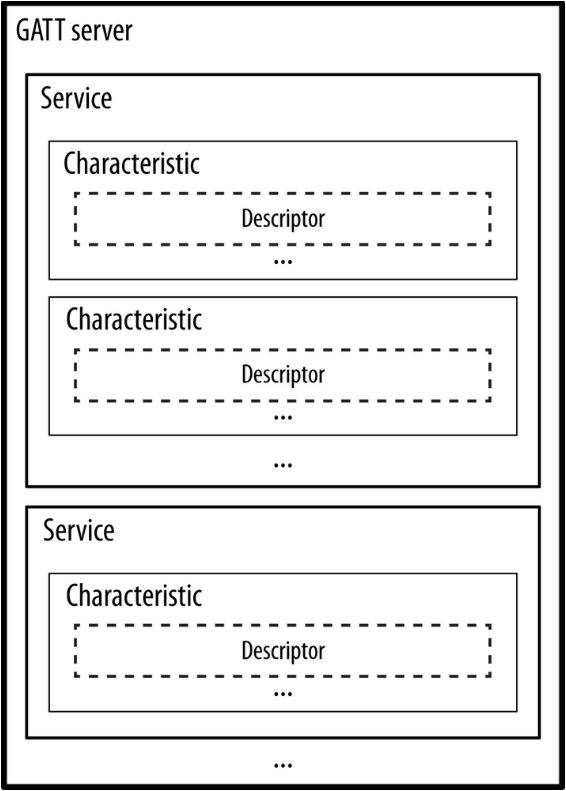
\includegraphics[width=0.5\textwidth,height=6cm,keepaspectratio=true]{images/gatt_service}
    \caption{
        The architecture of the GATT Server. Functionality is grouped as services. Services contain data as characteristics that can be read from or written to. Descriptors are used as metadata to describe characteristics and for configuring the server to notify the client of updates from the characteristic they are grouped under \cite{townsend_cufi}.
    }
    \label{fig:gatt_server}
\end{figure}

The \textit{Generic Attribute Profile} extends the functionality of ATT by creating a hierarchy and data abstraction model on top of it. The GATT server groups attributes into \textit{Services}. Services contain data points called \textit{Characteristics}. These characteristics can be interpreted and configured using fields called \textit{Descriptors}. See Figure \ref{fig:gatt_server} for a schematic layout of the GATT Server. 

\begin{figure}[]
    \centering
    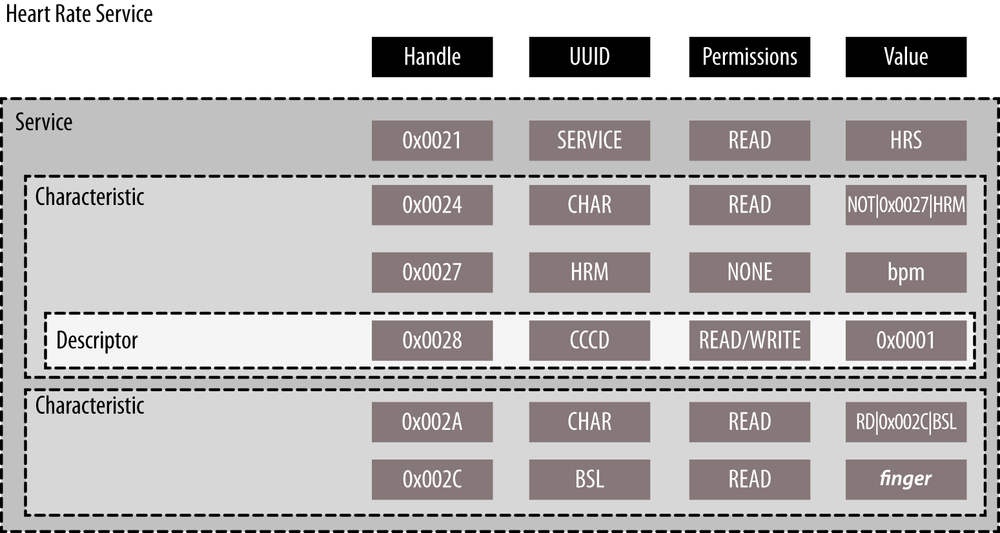
\includegraphics[width=0.5\textwidth,height=6cm,keepaspectratio=true]{images/heartrate_service}
    \caption{
        An example of a service. Each element is searchable through its UUID and then uniquely identifiable using its consecutively numbered handle \cite{townsend_cufi}.
    }
    \label{fig:hrs_layout}
\end{figure}
For a real-world example, see the Heart Rate Service (HRS) in Figure \ref{fig:hrs_layout}. The HRS allows a Client to read the heart rate sensor of a device. The HRS contains a characteristic called Heartrate. One of the descriptors tells us that the unit is defined as \textbf{beats per minute}. We could read the characteristic value manually, but if we would like to be notified when a new measurement is done, then we can set the Notify bit of the \textit{Client Characteristic Configuration} or CCC descriptor.

To be able to read or write to a characteristic, we need its handle. A handle is a number that is unique for a characteristic within a GATT Server. To find this handle, we can perform a \textit{Find By Type Request} using its 16-bit Universally Unique Identifier (UUID). Bluetooth SIG has predefined UUIDs for many predefined Services. Each predefined service has a specification that defines the shape of the service. This includes all the characteristics, descriptors, and their respective UUIDs.

The process of finding all these handles is what is called \textit{Service Discovery}. The result of this process is a list of handles that can be used to read and write to the server. After Service Discovery is done, the GATT Servers need to be configured. This usually means writing to the CCC descriptor to configure notifications for the desired characteristics. This process will, from here on, be referred to as Configuration. 

Both the Central and the Peripheral can be Servers and Clients at the same time. For example, a phone can provide the central time for a smartwatch to display on the watch face, while the smartwatch measures the heart rate for the phone to present within a health application. This means that a Service Discovery and Configuration need to be performed by both the Central and the Peripheral.

\section{Connection Setup}
As previously defined in Section \ref{sec:ch2_wireless_connection}, the connection setup starts from the Connection Request and ends when the last non-application packet is sent. The packets that occur during Connection Setup can be divided into four groups which correspond to the subjects discussed in the previous sections.
\begin{itemize}
    \item Link Layer
    \item Service Discovery
    \item Configuration
    \item Application
\end{itemize} 
The order in which they occur is usually Service Discover, Configuration, and then Application, with Link Layer communication starting parallel to the Service Discovery from the start.

\section{Operating Systems}
The FreeBie project was originally developed using the open-source BLE stack Packetcraft. Due to its architecture, it was especially suitable to be modified in the way required for intermittent operation. This is because all OS tasks are managed using a single scheduler which uses a generic sleep method. This sleep method was altered to configure the real-time clock (RTC), dump the memory to FRAM, and fully power down the SoC.

However, since FreeBie was originally developed, Packetcraft has gone into closed-source development. For this reason, a newer RTOS was chosen for the central. Zephyr OS is a modern RTOS developed by the Linux Foundation and is now the officially supported stack for Nordic Semiconductors.

**something extra about modifying link layer stack

\section{Demo Application}
To be able to benchmark the improvements proposed in this thesis we need a demo application. The network topology will be a simple Central / Peripheral network with a single peripheral. See Figure \ref{}